\chapter{ARN non codants et régulation post-transcriptionnelle}\label{ch:b3:rna-regulation}

En 1990, deux botanistes ont voulu rendre des pétunias d'un pourpre plus
soutenu en leur donnant des copies supplémentaires du gène de l'enzyme
du pigment. Près de la moitié des plantes transgéniques sont sorties
blanches, ou pourpres avec des secteurs blancs~: le gène ajouté avait
éteint la copie propre de la plante en même temps que lui-même. Huit
ans plus tard, deux généticiens du ver, en injectant de l'ARN dans
\emph{Caenorhabditis elegans}, ont trouvé qu'un ARN double brin
correspondant à un gène musculaire éteignait ce gène, chez le ver
injecté et dans sa descendance, bien plus puissamment que l'un ou
l'autre brin seul. Les deux énigmes avaient une même réponse~: la
cellule possède une machinerie qui se sert de courts ARN pour trouver
et réduire au silence les ARN de séquence complémentaire. Cette
machinerie, et plus largement tout ce qui advient à un ARN messager
après sa transcription --- comment il est épissé, où il est envoyé,
combien de temps il vit, s'il est traduit --- font l'objet de ce
chapitre. Le volume de première année traitait le gène comme une unité
allumée ou éteinte à son promoteur~; ici c'est le transcrit lui-même
qui devient l'objet du contrôle.

\section{Le recensement des ARN d'une cellule}

\begin{definition}[ARN non codant]\label{def:b3:rna-regulation:ncrna}
\index{ARN non codant}\index{microARN}\index{siARN}\index{piARN}\index{long ARN non codant}\index{petit ARN nucléaire}
Un \emph{ARN non codant} (ncARN) est un transcrit qui fonctionne en
tant qu'ARN et non comme matrice d'une protéine. Outre les ARN
ribosomiques et de transfert de la traduction et les \emph{petits ARN
nucléaires} (snARN) du spliceosome, une cellule eucaryote contient~:
des \emph{microARN} (miARN) de \numrange{21}{23} nucléotides, découpés
dans des tiges-boucles portées par ses propres transcrits et qui
guident la répression de messagers partiellement complémentaires~; des
\emph{petits ARN interférents} (siARN), de même longueur, découpés dans
de longs ARN double brin et qui guident le clivage de cibles
parfaitement appariées~; des \emph{ARN interagissant avec Piwi}
(piARN), de \numrange{26}{31} nucléotides, actifs dans la lignée
germinale contre les transposons~; de petits ARN nucléolaires qui
guident la modification des ARN ribosomiques~; et de \emph{longs ARN
non codants} (lncARN), transcrits de plus de \qty{200}{nt} sans cadre
de lecture ouvert digne de ce nom, dont \emph{\omterm{def:b3:chromatin-epigenetics:x-inactivation}{Xist}} du
\cref{ch:b3:chromatin-epigenetics} est le mieux compris. Les exons
codants représentent environ \qty{1.5}{\%} du génome humain~; une
grande partie du reste est transcrite à un moment ou un autre dans une
cellule ou une autre, mais quelle part de cette transcription est
fonctionnelle reste une question ouverte.
\end{definition}

\begin{remark}[L'abondance n'est pas la fonction]\label{rem:b3:rna-regulation:function}
Un transcrit peut être détecté parce que la polymérase fuit, et non
parce que l'ARN fait quelque chose~; la plupart des lncARN sont
présents à moins d'une copie par cellule, mal conservés et sans
conséquence lorsqu'on les supprime. Le critère de fonction est
génétique~: un phénotype lorsque l'ARN, et non seulement son ADN, est
retiré. \emph{\omterm{def:b3:chromatin-epigenetics:x-inactivation}{Xist}}, les miARN et les \omterm{def:b3:rna-regulation:ncrna}{piARN} le passent haut la main~;
des dizaines de milliers de lncARN annotés, quelques centaines l'ont
passé à ce jour.
\end{remark}

\section{L'interférence par ARN et les microARN}

\begin{definition}[Interférence par ARN]\label{def:b3:rna-regulation:rnai}
\index{interférence par ARN}\index{Dicer}\index{Argonaute}\index{RISC}
L'\emph{interférence par ARN} (ARNi) est la répression d'un gène,
spécifique de sa séquence, par un petit ARN dérivé d'un ARN double
brin. L'enzyme \emph{Dicer}, une RNase~III, découpe le long ARN double
brin en duplex de \numrange{21}{23} nucléotides à extrémités 3$'$
sortantes de deux nucléotides~; un brin de chaque duplex, le brin
guide, est chargé dans une protéine \emph{Argonaute} pour former le
\emph{complexe de silençage induit par l'ARN} (RISC). Le guide
s'apparie à un ARN cible complémentaire, et le domaine endonucléase
d'Argonaute coupe la cible en face des nucléotides 10 et 11 du guide~;
l'ARN coupé est ensuite dégradé et le RISC libéré pour en trouver un
autre. Chez les plantes, les vers et les champignons, une ARN
polymérase ARN-dépendante recopie la cible en un nouvel ARN double
brin, si bien que le signal est amplifié et se propage~; les mammifères
n'ont pas cette étape.
\end{definition}

\begin{proof}[Faits expérimentaux]
Napoli, Lemieux et Jorgensen (1990) ont introduit dans le pétunia une
copie supplémentaire du gène de la chalcone synthase pour intensifier
la couleur des fleurs~; \qty{42}{\%} des transformants sont sortis
blancs ou panachés, le transgène et le gène endogène étant tous deux
éteints --- la «~cosuppression~». Guo et Kemphues (1995) ont trouvé
qu'un ARN antisens dirigé contre un gène de \emph{C.~elegans}
l'éteignait, mais que le témoin sens le faisait aussi. Fire, Mello et
leurs collègues (1998) ont levé le paradoxe~: leurs préparations de
brins isolés étaient contaminées par des doubles brins, et l'ARN double
brin purifié d'\emph{unc-22} injecté à un ver donnait le phénotype
tremblant \emph{unc-22} à des concentrations de quelques molécules par
cellule, alors que l'ARN sens ou antisens pur ne donnait presque rien~;
la répression gagnait des tissus éloignés du point d'injection et
passait à la descendance. Hamilton et Baulcombe (1999) ont détecté les
ARN de \qty{25}{nt} dans les plantes éteintes, et Zamore et ses
collègues (2000) ont montré, dans un extrait de mouche, que l'ARN
double brin y est découpé et que la cible est clivée à intervalles de
\qty{21}{nt}.
\end{proof}

\begin{omfigure}
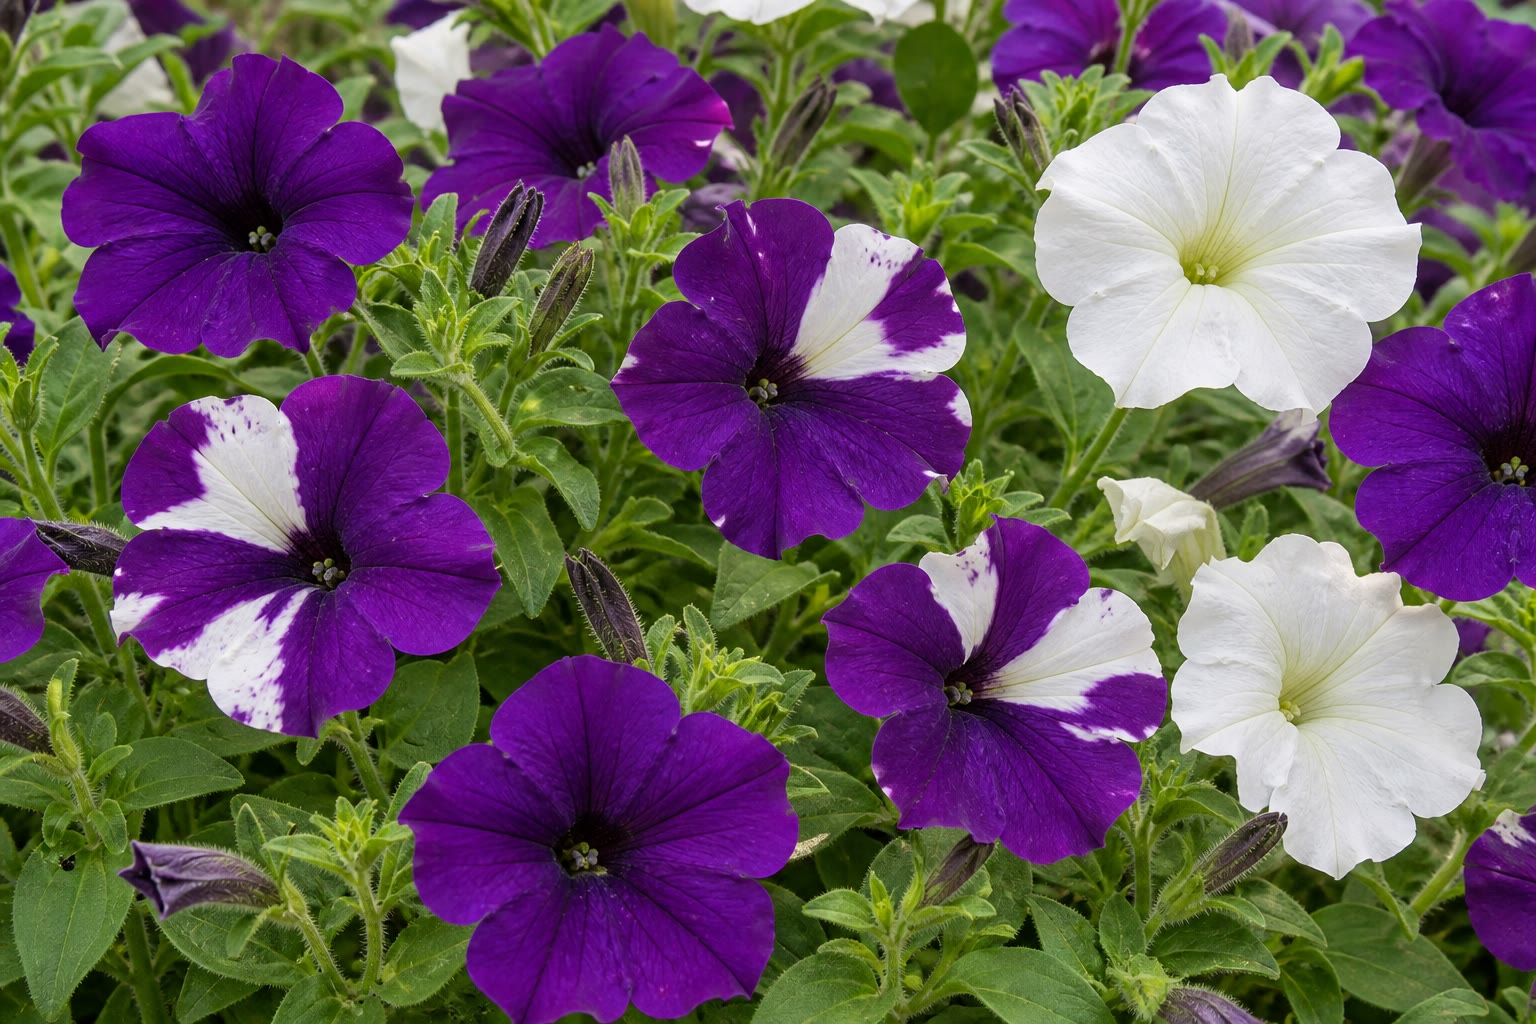
\includegraphics[width=0.46\linewidth]{images/book5/ai/b5-02-petunia-cosuppression.jpg}\hspace{0.04\linewidth}
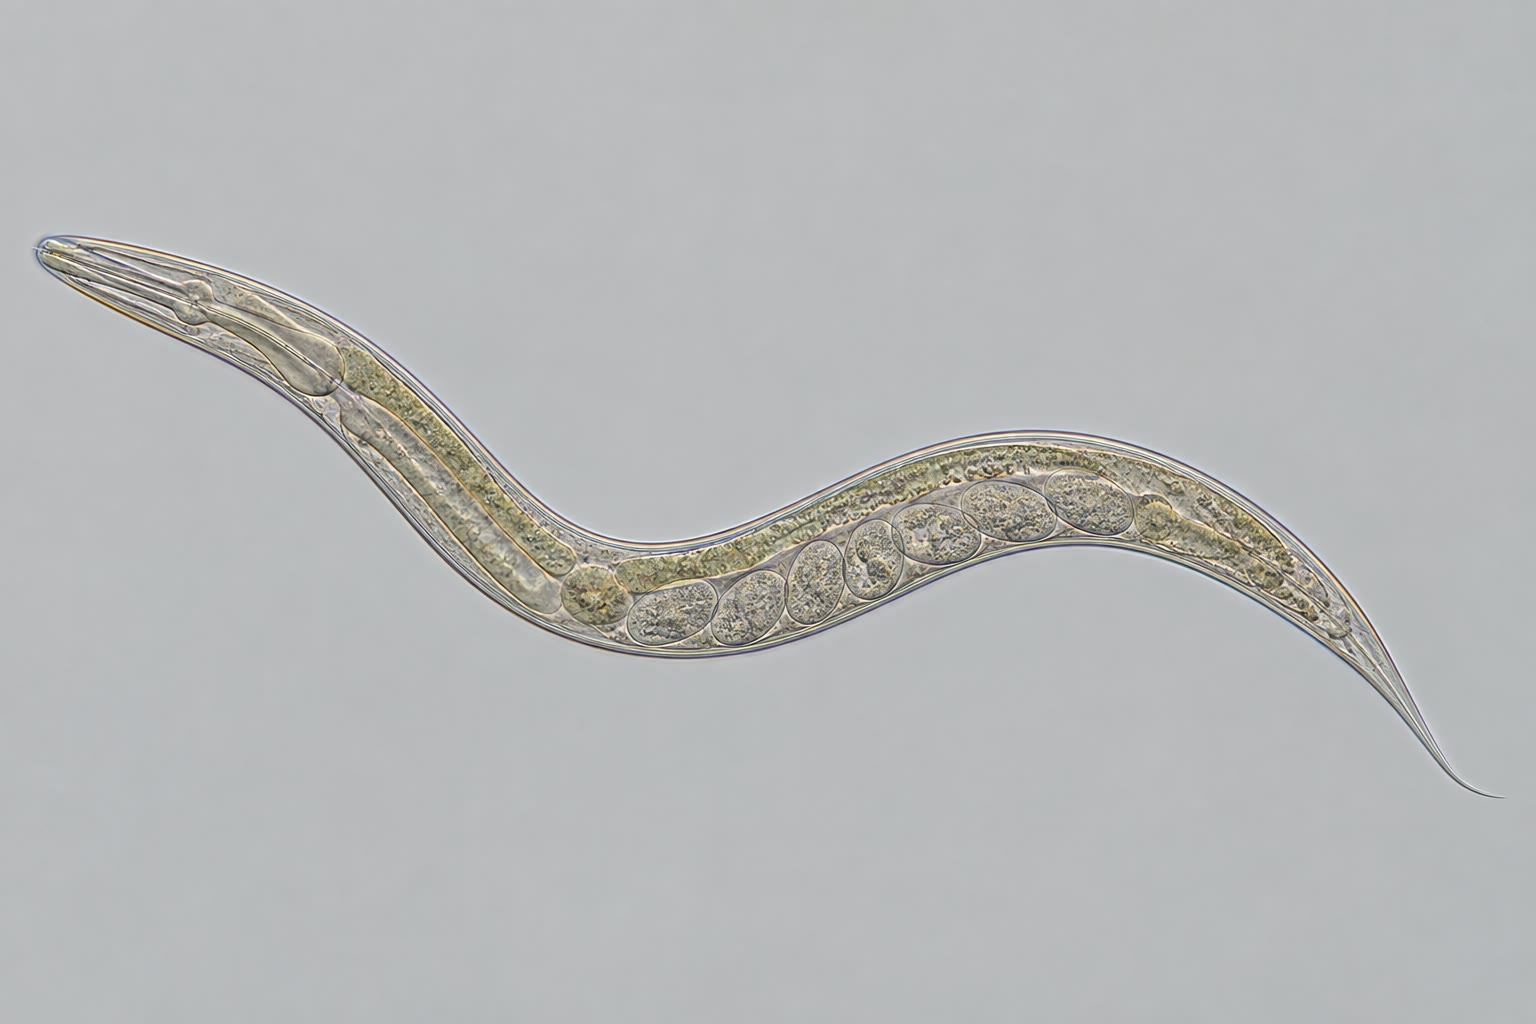
\includegraphics[width=0.46\linewidth]{images/book5/ai/b5-02-c-elegans.jpg}

{\small À gauche~: des pétunias porteurs d'un gène de pigment
supplémentaire, avec les secteurs blancs de la cosuppression. À
droite~: le nématode \emph{Caenorhabditis elegans}, long d'environ un
millimètre et transparent, chez qui un ARN double brin injecté a éteint
le gène correspondant dans l'animal entier et chez sa descendance.}
\end{omfigure}

\begin{definition}[Les microARN]\label{def:b3:rna-regulation:mirna}
\index{microARN!biogenèse}\index{Drosha}\index{séquence graine}
Un \emph{\omterm{def:b3:rna-regulation:ncrna}{microARN}} est codé dans le génome --- par un gène propre ou
par un intron d'un gène codant --- et transcrit par l'ARN polymérase~II
sous forme d'un long transcrit primaire (pri-miARN) contenant une
tige-boucle d'environ \qty{70}{nt}. Dans le noyau, la RNase~III
\emph{Drosha}, avec son partenaire DGCR8, découpe la tige-boucle
(le pré-miARN)~; l'exportine-5 la transporte dans le cytoplasme, où
\omterm{def:b3:rna-regulation:rnai}{Dicer} retire la boucle et laisse un duplex de \qty{22}{nt}. Un brin est
chargé dans \omterm{def:b3:rna-regulation:rnai}{Argonaute}. Le miARN mature reconnaît ses cibles surtout par
sa \emph{graine}, les nucléotides 2 à 8, qui s'apparie à des sites
situés le plus souvent dans la région 3$'$ non traduite d'un messager~;
le reste du miARN s'apparie imparfaitement, de sorte que la cible n'est
pas clivée mais réprimée~: le \omterm{def:b3:rna-regulation:rnai}{RISC} recrute des protéines qui
raccourcissent la queue poly(A), retirent la coiffe et inhibent la
traduction, et le messager est dégradé plus vite. Une graine ne faisant
que sept nucléotides, un miARN a des centaines de cibles, et plus de la
moitié des gènes codants humains portent des sites conservés pour au
moins l'un des quelques centaines de miARN humains bien établis.
\end{definition}

\begin{proof}[Faits expérimentaux]
\emph{lin-4}, un gène nécessaire au passage du ver de son premier stade
larvaire au second, s'est révélé chez Lee, Feinbaum et Ambros (1993)
coder non pas une protéine mais un ARN de \qty{22}{nt}, complémentaire
de sept sites de la région 3$'$ non traduite du messager de
\emph{lin-14}, le gène qu'il était connu pour réprimer. Lorsque la
larve entre dans le second stade, la protéine LIN-14 disparaît alors
que son ARNm demeure~: la répression est post-transcriptionnelle.
Reinhart et ses collègues (2000) ont trouvé un second ARN de ce type,
\emph{let-7}, qui commande les transitions larvaires suivantes~;
Pasquinelli (2000) a trouvé \emph{let-7} chez la mouche et chez
l'homme, avec la même séquence, ce qui a fait d'une curiosité du ver un
mécanisme général.
\end{proof}

\begin{omfigure}
\begin{tikzpicture}[every node/.style={font=\scriptsize}, >=stealth]
  % nucleus box
  \draw[rounded corners=8pt, thick, gray!60, fill=gray!6] (-0.4,-1.1) rectangle (5.2,2.7);
  \node[gray, anchor=south west] at (-0.3,-1.05) {noyau};
  % gene and pri-miRNA
  \draw[very thick, omDef] (0,2.0) -- (2.4,2.0); \node[above] at (1.2,2.05) {gène de miARN, Pol~II};
  \draw[->, thick] (1.2,1.85) -- (1.2,1.35);
  % hairpin
  \draw[thick, omThm!70!black] (0.2,1.0) -- (0.9,1.0) .. controls (1.0,1.0) and (1.05,0.9) .. (1.1,0.5) .. controls (1.15,0.1) and (1.25,0.1) .. (1.3,0.5) .. controls (1.35,0.9) and (1.4,1.0) .. (1.5,1.0) -- (2.2,1.0);
  \draw[thick, omThm!70!black] (1.1,0.5) -- (1.3,0.5);
  \node[below] at (1.2,0.0) {tige-boucle du pri-miARN};
  % Drosha
  \draw[thick, fill=omExo!35] (2.9,0.7) ellipse (0.55 and 0.28); \node at (2.9,0.7) {Drosha};
  \draw[->, thick] (2.3,0.85) -- (2.4,0.75);
  \draw[->, thick] (3.5,0.7) -- (4.2,0.7) node[midway, above] {coupure};
  % pre-miRNA
  \draw[thick, omThm!70!black] (4.3,0.9) .. controls (4.5,0.9) and (4.55,0.4) .. (4.6,0.1) .. controls (4.65,-0.2) and (4.75,-0.2) .. (4.8,0.1) .. controls (4.85,0.4) and (4.9,0.9) .. (5.1,0.9);
  \node[below, align=center] at (4.7,-0.25) {pré-miARN\\\qty{70}{nt}};
  % export
  \draw[->, thick] (5.35,0.4) -- (6.3,0.4) node[midway, above, xshift=0.2cm] {exportine-5};
  % cytoplasm
  \node[gray, anchor=north west] at (5.5,2.65) {cytoplasme};
  \draw[thick, fill=omExo!35] (6.9,0.4) ellipse (0.5 and 0.28); \node at (6.9,0.4) {Dicer};
  \draw[->, thick] (7.45,0.4) -- (8.1,0.4);
  \draw[thick, omThm!70!black] (8.2,0.55) -- (9.6,0.55); \draw[thick, omThm!70!black] (8.35,0.25) -- (9.75,0.25);
  \node[below, align=center] at (8.95,0.15) {duplex de \qty{22}{nt}};
  \draw[->, thick] (8.95,-0.4) -- (8.95,-0.9) node[midway, right] {un brin chargé};
  % RISC on mRNA
  \draw[thick, fill=omProp!35] (8.95,-1.45) ellipse (0.85 and 0.35); \node at (8.95,-1.45) {Argonaute};
  \draw[thick, omThm!70!black] (8.3,-1.85) -- (9.6,-1.85);
  \draw[very thick, omDef] (5.6,-2.15) -- (11.4,-2.15);
  \node[below] at (6.4,-2.2) {ARNm~: région codante}; \node[below] at (10.3,-2.2) {3$'$ UTR, site cible};
  \draw[omDef, thick] (11.4,-2.15) -- (11.8,-2.15) node[right] {AAAA};
  \draw[->, thick, omThm] (9.9,-1.5) -- (10.9,-1.5) node[right, align=left] {désadénylation,\\dégradation, moins\\de traduction};
  \node[below, align=center] at (8.95,-2.7) {la graine (nt 2--8)\\s'apparie au site};
\end{tikzpicture}

{\small Biogenèse d'un \omterm{def:b3:rna-regulation:ncrna}{microARN}. La tige-boucle est découpée dans le
transcrit primaire par \omterm{def:b3:rna-regulation:mirna}{Drosha} dans le noyau, exportée, taillée par
\omterm{def:b3:rna-regulation:rnai}{Dicer} en un duplex de \qty{22}{nt}, et un brin est chargé dans
\omterm{def:b3:rna-regulation:rnai}{Argonaute}. La graine s'apparie à un site de la région 3$'$ non traduite
d'un messager, et le messager est désadénylé, dégradé et moins traduit.}
\end{omfigure}

\begin{theorem}[Ce qu'un microARN fait au niveau et à la vitesse d'un messager]\label{thm:b3:rna-regulation:mirna-kinetics}
\index{demi-vie de l'ARNm}\index{temps de réponse}
Un messager est synthétisé à la vitesse constante $k$ et dégradé avec
la constante de vitesse du premier ordre $\gamma$~; un \omterm{def:b3:rna-regulation:ncrna}{microARN} présent
au niveau $R$ ajoute un terme de dégradation $\gamma' R\, m$. Le niveau
d'ARNm $m(t)$ obéit alors à
\[
\frac{\mathrm{d}m}{\mathrm{d}t} = k - (\gamma + \gamma' R)\, m,
\qquad
m^{*} = \frac{k}{\gamma + \gamma' R},
\qquad
m(t) = m^{*} + (m_{0} - m^{*})\,e^{-(\gamma + \gamma' R)t}.
\]
Le \omterm{def:b3:rna-regulation:ncrna}{microARN} abaisse l'état stationnaire d'un facteur $1 + \gamma' R/
\gamma$ et raccourcit du même facteur la constante de temps de toute
variation de $m$, qui passe de $1/\gamma$ à $1/(\gamma + \gamma' R)$.
Un gène réglé par un \omterm{def:b3:rna-regulation:ncrna}{microARN} est donc à la fois plus discret et plus
rapide~: il atteint plus tôt un nouvel état stationnaire après un
changement de son promoteur, et les fluctuations de sa transcription
sont amorties.
\end{theorem}
\begin{proof}
L'équation est linéaire à coefficients constants~; son point fixe est
$m^{*}$, où le membre de droite s'annule, et le changement de variable
$u = m - m^{*}$ donne $\mathrm{d}u/\mathrm{d}t = -(\gamma + \gamma' R)\,u$,
d'où l'exponentielle. Le temps de demi-approche vaut $\ln 2/(\gamma + \gamma'
R)$, et $\gamma = \ln 2 / t_{1/2}$ où $t_{1/2}$ est la demi-vie
naturelle du messager.
\end{proof}

\begin{example}[Une répression d'un facteur quatre]\label{ex:b3:rna-regulation:fourfold}
Un messager de demi-vie naturelle \qty{30}{min} ($\gamma =
\qty{0.023}{min^{-1}}$), transcrit à $k = 2$ molécules par minute, se
tient à $m^{*} = 2/0.023 \approx 87$ copies par cellule et met
\qty{30}{min} à parcourir la moitié du chemin vers un nouveau niveau
après un changement de son promoteur. Un \omterm{def:b3:rna-regulation:ncrna}{microARN} qui triple sa
constante de dégradation ($\gamma' R = 3\gamma$) le ramène à $22$
copies et ramène le temps de demi-approche à \qty{7.5}{min}. Les mêmes
nombres, lus à l'envers, montrent pourquoi l'invalidation d'un miARN
donne souvent des phénotypes discrets~: un facteur quatre sur un
messager lui-même tamponné en aval peut laisser l'organisme presque
normal, et l'effet ne se voit que sous contrainte ou dans la
chronologie.
\end{example}

\begin{omfigure}
\begin{tikzpicture}
\begin{axis}[
  width=0.7\linewidth, height=5.6cm,
  axis x line=bottom, axis y line=left,
  xmin=0, xmax=120, ymin=0, ymax=100,
  xlabel={temps après l'allumage du promoteur (min)}, ylabel={ARNm par cellule},
  xlabel style={font=\small, at={(axis description cs:0.5,-0.12)}, anchor=north},
  ylabel style={font=\small},
  tick label style={font=\small}, xtick={0,30,60,90,120}, ytick={0,22,50,87},
  clip=false,
]
\addplot[very thick, omDef, domain=0:120, samples=80] {87*(1-exp(-0.0231*x))};
\addplot[very thick, omThm, domain=0:120, samples=80] {21.7*(1-exp(-0.0924*x))};
\addplot[dashed, gray, domain=0:120, samples=2] {87};
\addplot[dashed, gray, domain=0:120, samples=2] {21.7};
\node[font=\scriptsize, omDef, anchor=south west] at (axis cs:5,90) {sans microARN~: $m^{*} = 87$, demi-approche \qty{30}{min}};
\node[font=\scriptsize, omThm, anchor=south west] at (axis cs:40,24) {avec microARN, $\gamma' R = 3\gamma$~: $m^{*} = 22$, demi-approche \qty{7.5}{min}};
\end{axis}
\end{tikzpicture}

{\small Montée d'un messager après l'allumage de son promoteur, avec
les nombres de l'\cref{ex:b3:rna-regulation:fourfold}. Le \omterm{def:b3:rna-regulation:ncrna}{microARN}
abaisse le plateau d'un facteur quatre et l'atteint quatre fois plus tôt.}
\end{omfigure}

\begin{method}[Éteindre un gène par ARN interférence]\label{met:b3:rna-regulation:knockdown}
\index{extinction de gène}\index{ARN en épingle à cheveux}
Pour réduire un gène au silence sans toucher à son ADN~: (1) choisir
une séquence de \qty{21}{nt} propre à son messager, en évitant les
correspondances de graine avec d'autres gènes~; (2) l'apporter sous
forme d'un duplex de \omterm{def:b3:rna-regulation:ncrna}{siARN} de synthèse (transitoire, quelques jours) ou
d'un \omterm{met:b3:rna-regulation:knockdown}{ARN en épingle à cheveux} court (shARN) exprimé par un vecteur, que
\omterm{def:b3:rna-regulation:rnai}{Dicer} traite en continu~; chez le ver, nourrir les animaux de bactéries
exprimant l'ARN double brin~; (3) mesurer le messager par PCR
quantitative et la protéine par immunoempreinte, en attendant une perte
de \qtyrange{70}{95}{\%} plutôt que l'absence complète d'une
invalidation~; (4) contrôler les effets hors cible par un second \omterm{def:b3:rna-regulation:ncrna}{siARN}
non chevauchant et par un sauvetage à l'aide d'une version du gène
résistante à l'ARNi. Une extinction est une perte de fonction
partielle et réversible~; les thérapies géniques aujourd'hui autorisées
sur ce principe apportent des \omterm{def:b3:rna-regulation:ncrna}{siARN} dirigés contre des messagers
hépatiques (transthyrétine, PCSK9) couplés à un sucre que
l'hépatocyte capte.
\end{method}

\section{Les petits ARN qui gardent le génome}

\begin{definition}[piARN et répression des transposons]\label{def:b3:rna-regulation:pirna}
\index{piARN!ping-pong}\index{répression des transposons}\index{dysgénésie hybride}
Les \emph{\omterm{def:b3:rna-regulation:ncrna}{piARN}} sont des ARN de \numrange{26}{31} nucléotides,
produits sans \omterm{def:b3:rna-regulation:rnai}{Dicer} à partir de longs transcrits simple brin d'\emph{amas
de \omterm{def:b3:rna-regulation:ncrna}{piARN}} génomiques --- des cimetières de copies défectueuses de
transposons --- et chargés sur la sous-famille PIWI des protéines
\omterm{def:b3:rna-regulation:rnai}{Argonaute}, dans la lignée germinale. Un \omterm{def:b3:rna-regulation:ncrna}{piARN} antisens d'un transposon
guide le clivage des transcrits de ce transposon~; le fragment clivé
devient un nouveau \omterm{def:b3:rna-regulation:ncrna}{piARN} sens, qui à son tour coupe les transcrits de
l'amas pour fabriquer d'autres \omterm{def:b3:rna-regulation:ncrna}{piARN} antisens --- le cycle
\emph{ping-pong}, amplification qui vise précisément le transposon
actif du moment. Des protéines PIWI nucléaires dirigent en outre la
méthylation de H3K9 et la \omterm{def:b3:chromatin-epigenetics:methylation}{méthylation de l'ADN} sur les copies
génomiques du transposon, reliant l'ARN aux marques de \omterm{def:b3:chromatin-epigenetics:nucleosome}{chromatine} du
\cref{ch:b3:chromatin-epigenetics}. Une mère dépose ses \omterm{def:b3:rna-regulation:ncrna}{piARN} dans
l'ovocyte~; une femelle dont la lignée n'a jamais rencontré un
transposon n'a pas de \omterm{def:b3:rna-regulation:ncrna}{piARN} contre lui, et sa descendance issue d'un
mâle porteur est stérile --- c'est la \emph{dysgénésie hybride}, vue
d'abord dans des croisements de \emph{drosophiles} entre souches de
laboratoire et souches sauvages.
\end{definition}

\begin{proposition}[Répression de la chromatine dirigée par l'ARN]\label{prop:b3:rna-regulation:rddm}
\index{méthylation de l'ADN dirigée par ARN}
Chez les plantes, une voie dédiée --- l'ARN polymérase~IV transcrit un
locus, une ARN polymérase ARN-dépendante en fait un double brin, un
\omterm{def:b3:rna-regulation:rnai}{Dicer} découpe des \omterm{def:b3:rna-regulation:ncrna}{siARN} de \qty{24}{nt}, \omterm{def:b3:rna-regulation:rnai}{Argonaute}~4 les ramène sur les
transcrits naissants de la polymérase~V au même locus et recrute la
méthyltransférase DRM2 --- méthyle l'ADN des transposons et des
séquences répétées~; c'est le mécanisme de la paramutation. Chez la
levure à fission, des \omterm{def:b3:rna-regulation:ncrna}{siARN} issus des répétitions centromériques
recrutent la méthyltransférase de H3K9 et bâtissent l'\omterm{def:b3:chromatin-epigenetics:nucleosome}{hétérochromatine}
dont le centromère a besoin. Dans les deux cas un ARN trouve une place
du génome par complémentarité et une marque de \omterm{def:b3:chromatin-epigenetics:nucleosome}{chromatine} y est
écrite~: spécifique de la séquence, auto-entretenue, et héritable au
travers des divisions.
\end{proposition}

\section{La vie d'un messager}

\begin{definition}[Épissage régulé]\label{def:b3:rna-regulation:splicing}
\index{épissage alternatif!régulation}\index{protéine SR}\index{hnRNP}\index{saut d'exon}
L'épissage alternatif produit des messagers différents à partir d'un
seul gène, par \emph{saut d'exon}, par le choix entre des exons
mutuellement exclusifs, par la rétention d'un intron ou par l'emploi de
sites d'épissage 5$'$ ou 3$'$ de rechange. Il est réglé par des
protéines de liaison à l'ARN qui reconnaissent des éléments de séquence
dans les exons et les introns voisins d'un site d'épissage~: les
\emph{protéines SR} fixées sur des amplificateurs exoniques recrutent
le spliceosome et favorisent l'inclusion de l'exon, les protéines
\emph{hnRNP} fixées sur des silenceurs la bloquent, et l'issue dans une
cellule donnée est fixée par les quantités relatives des deux familles.
Plus de \qty{90}{\%} des gènes humains à plusieurs exons subissent un
épissage alternatif~; le gène \emph{Dscam} de la \emph{drosophile},
avec ses quatre blocs d'exons mutuellement exclusifs (12, 48, 33 et 2
possibilités), peut produire \num{38016} protéines distinctes, chaque
neurone en exprimant un jeu différent qui permet à ses branches de se
reconnaître et de s'éviter.
\end{definition}

\begin{proof}[Faits expérimentaux]
Le sexe d'une mouche est décidé par une cascade d'épissages. Chez la
femelle, le gène \emph{Sex-lethal} (\emph{Sxl}) fabrique une protéine
fonctionnelle~; SXL est une protéine de liaison à l'ARN qui bloque un
site d'épissage dans son propre transcrit (de sorte qu'un exon porteur
d'un codon stop est sauté et que la protéine continue d'être produite)
et dans le transcrit de \emph{transformer}, ce qui impose l'épissage
femelle~; TRA, avec TRA-2, se fixe ensuite sur un amplificateur exonique
du transcrit de \emph{doublesex} et dirige la forme femelle du facteur
de transcription DSX. Chez le mâle, faute de SXL, chacun de ces
transcrits prend l'épissage par défaut, \emph{transformer} contient un
codon stop, et DSX sort sous la forme mâle. Tout caractère sexuellement
dimorphe de la mouche découle du DSX produit~; une femelle dont
\emph{tra} est muté se développe en mâle.
\end{proof}

\begin{definition}[Stabilité et localisation des ARNm]\label{def:b3:rna-regulation:stability}
\index{élément riche en AU}\index{localisation des ARNm}\index{élément de réponse au fer}
La \emph{demi-vie} d'un messager va de la minute au jour et est fixée
par des éléments de sa région 3$'$ non traduite. Les \emph{éléments
riches en AU} (répétitions AUUUA) des messagers de cytokines, de
facteurs de croissance et de proto-oncogènes sont reconnus par des
protéines qui recrutent des désadénylases et donnent des demi-vies de
\qtyrange{10}{30}{min}, si bien qu'une bouffée de transcription produit
une bouffée de protéine et rien de plus~; les mutations qui les
suppriment causent une surexpression et, pour certains
proto-oncogènes, un cancer. Les \emph{éléments de localisation},
souvent structurés, sont reconnus par des adaptateurs qui relient le
messager à un moteur~: les messagers de \emph{bicoid} et d'\emph{oskar}
sont portés aux deux pôles de l'œuf de mouche par la dynéine et la
kinésine sur les microtubules, le messager de la $\beta$-actine au bord
avant d'un fibroblaste, et les messagers des protéines synaptiques dans
les dendrites, où ils sont traduits à la demande. L'\emph{élément de
réponse au fer} (IRE), une tige-boucle reconnue par les protéines
régulatrices du fer IRP1 et IRP2 quand le fer est rare, fait deux
travaux opposés depuis deux positions~: dans la région 5$'$ non
traduite du messager de la ferritine, l'IRP fixée bloque le ribosome~;
dans la région 3$'$ non traduite du messager du récepteur de la
transferrine, l'IRP fixée protège le transcrit d'une nucléase.
\end{definition}

\begin{example}[Le fer, lu par une seule tige-boucle]\label{ex:b3:rna-regulation:iron}
Quand le fer est bas, l'IRP se fixe sur les deux messagers~: la
ferritine, protéine de stockage, n'est pas traduite, et le récepteur de
la transferrine, qui importe le fer, est stabilisé et abondant --- la
cellule stocke moins et importe plus. Quand le fer est haut, il
convertit IRP1 en aconitase (elle acquiert un centre fer--soufre et
perd son affinité pour l'ARN) et déclenche la dégradation d'IRP2~: la
ferritine est traduite, le messager du récepteur se dégrade en quelques
minutes, et la cellule stocke plus et importe moins. Aucun changement
de transcription n'est nécessaire. Une mutation ponctuelle de l'IRE de
la ferritine qui empêche la fixation de l'IRP cause une synthèse
constitutive de ferritine et le syndrome héréditaire
hyperferritinémie--cataracte.
\end{example}

\begin{omfigure}
\begin{tikzpicture}[every node/.style={font=\scriptsize}, >=stealth]
  \foreach \yy/\state in {2.2/fer bas, -0.9/fer haut} {
    \node[left, font=\small\bfseries] at (-0.2,\yy+0.35) {\state};
    % ferritin mRNA
    \draw[very thick, omDef] (0.3,\yy+0.6) -- (4.6,\yy+0.6); \node[below] at (3.3,\yy+0.4) {ARNm de la ferritine};
    \draw[thick, omThm!70!black] (0.9,\yy+0.6) .. controls (0.9,\yy+1.15) and (1.3,\yy+1.15) .. (1.3,\yy+0.6); \node[below] at (1.1,\yy+0.55) {IRE};
    \draw[fill=omDef!20, thick] (2.2,\yy+0.42) rectangle (4.4,\yy+0.78);
    % TfR mRNA
    \draw[very thick, omDef] (6.2,\yy+0.6) -- (10.6,\yy+0.6); \node[below, font=\tiny] at (7.1,\yy+0.4) {ARNm du récepteur de la transferrine};
    \draw[fill=omDef!20, thick] (6.4,\yy+0.42) rectangle (8.6,\yy+0.78);
    \foreach \x in {9.0,9.5,10.0} \draw[thick, omThm!70!black] (\x,\yy+0.6) .. controls (\x,\yy+1.1) and (\x+0.35,\yy+1.1) .. (\x+0.35,\yy+0.6);
    \node[below, font=\tiny] at (9.9,\yy+0.55) {IRE (3$'$ UTR)};
  }
  % low iron: IRP bound
  \draw[thick, fill=omProp!40] (1.1,3.35) ellipse (0.4 and 0.24); \node at (1.1,3.35) {IRP};
  \node[right, omThm] at (1.55,3.35) {ribosome bloqué~: pas de ferritine};
  \foreach \x in {9.18,9.68,10.18} { \draw[thick, fill=omProp!40] (\x,3.35) ellipse (0.28 and 0.2); }
  \node[above, omMeth!70!black] at (9.7,3.75) {protégé de la nucléase~: récepteur stable et abondant};
  \node[below, omMeth!70!black] at (1.1,1.75) {stocke moins};
  \node[below, omMeth!70!black] at (7.4,1.75) {importe plus};
  % high iron: IRP off
  \node[right, omMeth!70!black] at (1.55,0.25) {traduit~: ferritine produite};
  \node[right, omThm, align=left] at (10.7,-0.3) {nucléase~:\\l'ARNm se dégrade};
  \node[below, omThm] at (1.1,-1.35) {stocke plus};
  \node[below, omThm] at (7.4,-1.35) {importe moins};
\end{tikzpicture}

{\small L'\omterm{def:b3:rna-regulation:stability}{élément de réponse au fer}. Quand le fer est bas, la protéine
régulatrice du fer se fixe sur les tiges-boucles IRE~: à l'extrémité
5$'$ du messager de la ferritine elle bloque la traduction, à
l'extrémité 3$'$ du messager du récepteur de la transferrine elle
bloque une nucléase. Quand le fer est haut la protéine les libère tous
deux~: la ferritine est produite, le messager du récepteur se dégrade.}
\end{omfigure}

\begin{proposition}[Contrôle traductionnel]\label{prop:b3:rna-regulation:translation}
\index{contrôle traductionnel}\index{eIF2}\index{riborégulateur}\index{cadre de lecture ouvert en amont}
L'initiation est le point de contrôle habituel de la traduction. La
phosphorylation du facteur d'initiation \emph{eIF2} par des kinases
qui détectent une carence en acides aminés, des protéines mal repliées,
un ARN double brin viral ou un manque d'hème arrête l'initiation
générale en quelques minutes, en épargnant quelques messagers dotés de
particularités --- notamment ceux qui portent des \emph{\omterm{prop:b3:rna-regulation:translation}{cadres de
lecture ouverts en amont}}, courts cadres de lecture de la région 5$'$
non traduite, qui piègent normalement les ribosomes et que la contrainte
fait contourner, de sorte que les facteurs de réponse au stress (GCN4
chez la levure, ATF4 chez les mammifères) sont produits précisément
quand tout le reste ne l'est pas. Le facteur de liaison à la coiffe
eIF4E est maintenu inactif par les protéines 4E-BP jusqu'à ce que la
kinase de signalisation de croissance mTOR les phosphoryle~: une
cellule ne traduit à plein régime que si les nutriments et les facteurs
de croissance le lui disent. Chez les bactéries, les
\emph{riborégulateurs} y parviennent sans aucune protéine~: une région
5$'$ structurée fixe un métabolite (pyrophosphate de thiamine,
S-adénosylméthionine, une purine) et, en le fixant, se replie autrement
pour enfouir le site de fixation du ribosome ou former un terminateur
de transcription, de sorte qu'un opéron de biosynthèse s'éteint quand
son produit est abondant.
\end{proposition}

\begin{omfigure}
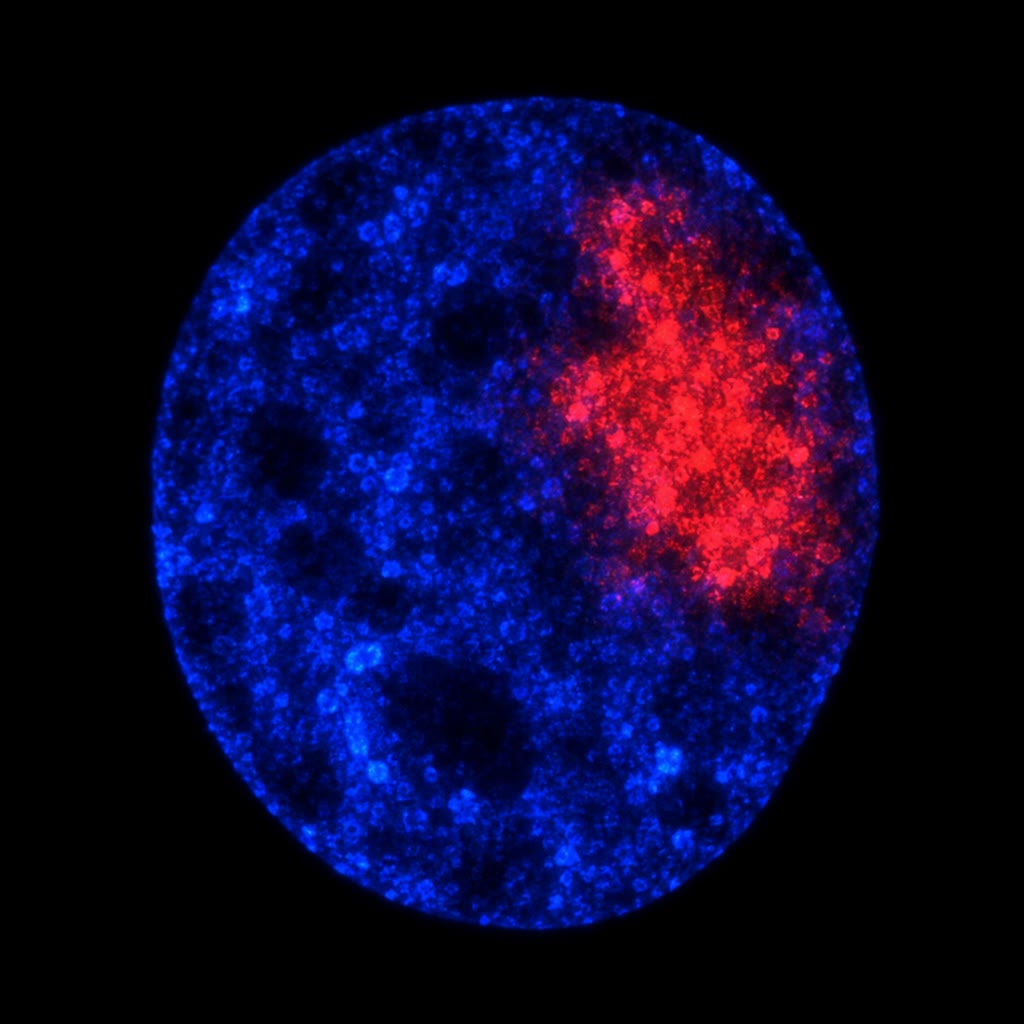
\includegraphics[width=0.36\linewidth]{images/book5/ai/b5-02-lncrna-nucleus.jpg}

{\small Un \omterm{def:b3:rna-regulation:ncrna}{long ARN non codant} à l'œuvre~: le transcrit \emph{\omterm{def:b3:chromatin-epigenetics:x-inactivation}{Xist}}
(rouge), détecté par hybridation fluorescente, recouvre le territoire
d'un chromosome~X dans un noyau de femelle (ADN en bleu).}
\end{omfigure}

\begin{remark}[Ce que rapporte le contrôle post-transcriptionnel]\label{rem:b3:rna-regulation:why}
Le contrôle transcriptionnel passe par le noyau, avec un délai de
quelques minutes à quelques heures avant qu'un nouveau messager soit
produit, exporté et traduit. Le contrôle du messager lui-même agit là
où la protéine est nécessaire, en quelques secondes à quelques minutes,
et il peut être local~: une seule dendrite traduisant un messager à une
seule synapse, le bord avant d'un fibroblaste fabriquant de l'actine là
où il rampe. Il fait en outre d'un gène plusieurs protéines, et permet
à un seul signal --- le fer, un acide aminé, un \omterm{def:b3:rna-regulation:ncrna}{microARN} --- de
coordonner des centaines de messagers à la fois sans toucher au moindre
promoteur.
\end{remark}

\section{Exercices}

\begin{exercise}[$\star$]\label{exo:b3:rna-regulation:1}
Distinguer miARN, \omterm{def:b3:rna-regulation:ncrna}{siARN} et \omterm{def:b3:rna-regulation:ncrna}{piARN} par leur origine, leur longueur, leur
dépendance à \omterm{def:b3:rna-regulation:rnai}{Dicer} et ce qu'ils font à leurs cibles.
\end{exercise}

\begin{exercise}[$\star$]\label{exo:b3:rna-regulation:2}
Retracer la biogenèse d'un \omterm{def:b3:rna-regulation:ncrna}{microARN} depuis son gène jusqu'à un messager
réprimé, en nommant l'enzyme de chaque coupure.
\end{exercise}

\begin{exercise}[$\star$]\label{exo:b3:rna-regulation:3}
Pourquoi l'injection d'ARN sens d'\emph{unc-22} à des vers
éteignait-elle le gène dans les premières expériences, et qu'ont changé
Fire et Mello~?
\end{exercise}

\begin{exercise}[$\star$]\label{exo:b3:rna-regulation:4}
Qu'advient-il de la ferritine et du récepteur de la transferrine
lorsqu'une cellule est privée de fer~? Quelle étape de l'expression est
contrôlée dans chaque cas~?
\end{exercise}

\begin{exercise}[$\star\star$]\label{exo:b3:rna-regulation:5}
Un messager a une demi-vie de \qty{2}{h} et est produit à $5$ molécules
par minute. Calculer son niveau stationnaire, puis le niveau et le
temps de demi-approche lorsqu'un \omterm{def:b3:rna-regulation:ncrna}{microARN} double sa constante de
dégradation.
\end{exercise}

\begin{exercise}[$\star\star$]\label{exo:b3:rna-regulation:6}
Une graine de sept nucléotides s'apparie à une séquence aléatoire avec
la probabilité $4^{-7}$. Dans un jeu de \num{20000} messagers dont les
régions 3$'$ non traduites mesurent en moyenne \qty{1000}{nt}, combien
de sites une graine de \omterm{def:b3:rna-regulation:ncrna}{microARN} rencontre-t-elle par hasard~? Qu'est-ce
qui distingue alors une vraie cible~?
\end{exercise}

\begin{exercise}[$\star\star$]\label{exo:b3:rna-regulation:7}
Prévoir le sexe d'une mouche (a) porteuse d'une mutation de perte de
fonction de \emph{tra} et de deux chromosomes~X~; (b) exprimant TRA
depuis un transgène constitutif, avec un seul X~; (c) totalement
dépourvue de \emph{dsx}.
\end{exercise}

\begin{exercise}[$\star\star$]\label{exo:b3:rna-regulation:8}
Le messager d'un proto-oncogène a normalement une demi-vie de
\qty{15}{min} à cause d'un \omterm{def:b3:rna-regulation:stability}{élément riche en AU}. Une translocation
chromosomique enlève l'élément et la demi-vie passe à \qty{3}{h}. De
quel facteur le niveau de protéine monte-t-il, si la traduction et la
dégradation des protéines sont inchangées~? Pourquoi est-ce oncogène
alors que la protéine est normale~?
\end{exercise}

\begin{exercise}[$\star\star$]\label{exo:b3:rna-regulation:9}
Une souche de laboratoire de \emph{drosophile} est dépourvue d'éléments
P~; une souche sauvage en porte. Prévoir la fertilité de la descendance
de (a) femelles de laboratoire $\times$ mâles sauvages, (b) femelles
sauvages $\times$ mâles de laboratoire, et expliquer l'asymétrie par
les \omterm{def:b3:rna-regulation:ncrna}{piARN}.
\end{exercise}

\begin{exercise}[$\star\star\star$]\label{exo:b3:rna-regulation:10}
À l'aide du \cref{thm:b3:rna-regulation:mirna-kinetics}, montrer que la
protéine issue d'un messager fluctue moins, en valeur relative, lorsque
le messager est sous contrôle d'un \omterm{def:b3:rna-regulation:ncrna}{microARN}, à niveau moyen de messager
égal. (La protéine moyenne le messager sur sa propre durée de vie, et
le messager se renouvelle plus vite.) Pourquoi une cellule paierait-elle
un \omterm{def:b3:rna-regulation:ncrna}{microARN} et une transcription plus forte pour obtenir la même
moyenne~?
\end{exercise}

\begin{exercise}[$\star\star\star$]\label{exo:b3:rna-regulation:11}
Chez le ver, une ARN polymérase ARN-dépendante fabrique des \omterm{def:b3:rna-regulation:ncrna}{siARN}
secondaires à partir du messager cible~; chez les mammifères, il n'y en
a pas. Prévoir, pour chacun, si la répression obtenue par une seule
injection d'ARN double brin dure au travers de nombreuses divisions
cellulaires et si elle se propage à d'autres tissus, et expliquer la
conséquence médicale pour les médicaments à \omterm{def:b3:rna-regulation:ncrna}{siARN}.
\end{exercise}

\begin{exercise}[$\star\star\star$]\label{exo:b3:rna-regulation:12}
Un lncARN nouvellement annoté est exprimé dans le cœur. Concevoir les
expériences qui distingueraient (a) un ARN fonctionnel, (b) un acte de
transcription fonctionnel dont l'ARN est sans importance, et (c) du
bruit, et dire ce que chacune prédit dans les trois cas.
\end{exercise}

\section{Problème~: l'horloge d'un ver}

\begin{problem}[{Problème du week-end --- l'interrupteur
\emph{lin-4}/\emph{lin-14} du ver chronométré par la cinétique du
messager, un ARN injecté puis dilué par les divisions d'un embryon et
sauvé par l'amplification, le régulon du fer quantifié et un
dénombrement d'épissages, pour finir sur le facteur de répression, le
temps de demi-basculement et le nombre de divisions que survit un
signal non amplifié}]
\label{pb:b3:rna-regulation:1}
Données~: le messager de \emph{lin-14} est produit à $k = 3$ molécules
par minute et par cellule et a une demi-vie de \qty{40}{min}. La
protéine LIN-14 est produite à $\beta = 2$ par messager et par minute
et a une demi-vie de \qty{3}{h}. À partir du début du second stade
larvaire, l'ARN \emph{lin-4} s'accumule et ajoute au messager un terme
de dégradation $\gamma' R = 3\gamma$ et, en bloquant l'initiation,
divise $\beta$ par deux. Un embryon de ver passe d'une cellule à
environ \num{550} cellules à l'éclosion~; un adulte a \num{959}
cellules somatiques.

\medskip
\noindent\textbf{Partie I --- Le messager.}
\begin{enumerate}
  \item Calculer $\gamma$ et le niveau stationnaire du messager
        \emph{lin-14} avant l'apparition de \emph{lin-4}.
  \item Calculer la constante de dégradation de la protéine et le
        niveau stationnaire de la protéine LIN-14.
  \item Une fois \emph{lin-4} présent, calculer le nouveau niveau de
        messager et la nouvelle constante de temps du messager.
  \item Calculer le nouvel état stationnaire de la protéine, et le
        facteur global de répression sur la protéine.
  \item Combien de temps après l'apparition de \emph{lin-4} le messager
        parcourt-il la moitié du chemin vers son nouveau niveau~? Et la
        protéine~? Quelle étape limite la vitesse du basculement~?
  \item Les expériences d'origine trouvaient la protéine disparue alors
        que l'ARNm était encore détectable. Est-ce compatible avec vos
        nombres~? Quelle fraction du messager subsiste~?
\end{enumerate}

\medskip
\noindent\textbf{Partie II --- Dilution et amplification.}
\begin{enumerate}[resume]
  \item On injecte dans la gonade d'un ver $10^{6}$ molécules d'ARN
        double brin, qui se répartissent également entre \num{250}
        œufs. Combien de molécules par œuf~?
  \item Si les molécules étaient simplement réparties à chaque
        division, combien chaque cellule du jeune ver de \num{550}
        cellules en garderait-elle~? Au bout de combien de divisions
        supplémentaires la moyenne passerait-elle sous une par cellule~?
  \item Fire et Mello ont vu la répression dans l'animal entier et dans
        sa descendance, à quelques molécules par cellule. Expliquer ce
        qu'une ARN polymérase ARN-dépendante ajoute à ce compte, et
        pourquoi l'effet s'estompe malgré tout au bout de quelques
        générations.
  \item Dans une cellule de mammifère, dépourvue d'une telle
        polymérase, une transfection de \omterm{def:b3:rna-regulation:ncrna}{siARN} dépose \num{5000} duplex
        dans une cellule qui se divise chaque jour~; le \omterm{def:b3:rna-regulation:rnai}{RISC} est stable
        mais se dilue par division. Au bout de combien de jours le
        compte passe-t-il sous \num{100}, à peu près le nombre
        nécessaire à une répression efficace~?
  \item Un \omterm{def:b3:rna-regulation:ncrna}{siARN} thérapeutique dirigé contre un messager hépatique est
        administré une fois et agit six mois. Les hépatocytes se
        divisent rarement. Expliquer pourquoi le mécanisme de la
        question 10 ne le limite pas, et ce qui le limite.
  \item Une graine de sept nucléotides s'apparie au hasard une fois
        tous les $4^{7}$ nucléotides. Le transcriptome du ver compte
        environ \qty{20}{Mb} de séquence 3$'$ non traduite. Combien de
        correspondances de graine dues au hasard \emph{lin-4} a-t-il,
        et comment les généticiens ont-ils su quelle cible comptait~?
\end{enumerate}

\medskip
\noindent\textbf{Partie III --- Le régulon du fer.}
\begin{enumerate}[resume]
  \item Dans une cellule riche en fer, le messager du récepteur de la
        transferrine a une demi-vie de \qty{10}{min}~; avec l'IRP
        fixée, \qty{50}{min}. À transcription inchangée, de quel
        facteur le messager monte-t-il quand le fer devient rare~?
  \item Le messager de la ferritine ne change pas de niveau, mais sa
        traduction tombe de $1$ à $0.05$ protéine par messager et par
        minute quand l'IRP se fixe. De quel facteur la synthèse de
        ferritine baisse-t-elle~?
  \item Combiner les deux~: de quel facteur le rapport de la capacité
        d'importation à la capacité de stockage change-t-il entre
        l'état riche et l'état pauvre en fer~?
  \item La protéine IRP1 est soit une protéine de liaison à l'ARN, soit
        une aconitase, selon qu'elle porte ou non un centre
        fer--soufre. Expliquer pourquoi cela en fait un capteur du fer
        lui-même et non d'une hormone.
  \item Un patient porte une mutation de l'IRE de la ferritine qui
        abolit la fixation de l'IRP. Prévoir le taux de ferritine, le
        fer sérique, et pourquoi le cristallin est atteint.
  \item Expliquer en une phrase pourquoi une même tige-boucle peut
        activer à une position et réprimer à une autre.
  \item IRP2 n'a pas de centre fer--soufre~; quand le fer est haut,
        elle est détruite par une ubiquitine-ligase dont la stabilité
        exige elle-même du fer et du dioxygène. Pourquoi une cellule
        garderait-elle deux capteurs de chimie si différente~?
\end{enumerate}

\medskip
\noindent\textbf{Partie IV --- Compter les isoformes.}
\begin{enumerate}[resume]
  \item \emph{Dscam} a des blocs d'exons offrant 12, 48, 33 et 2
        possibilités mutuellement exclusives. Combien d'isoformes~? Si
        chaque neurone en exprime environ $50$ au hasard, quelle est la
        probabilité que deux neurones donnés en partagent au moins
        une~? (Utiliser $1 - (1 -
        50/N)^{50}$.)
  \item Pourquoi un neurone gagne-t-il à posséder des isoformes que ses
        voisins n'ont presque sûrement pas~?
  \item Un gène à $n$ exons cassettes, chacun inclus ou sauté de façon
        indépendante, donne combien de messagers~? Combien pour
        $n = 10$~? Pourquoi le nombre réel dans un type cellulaire
        donné est-il bien plus petit~?
  \item Chez la mouche, pourquoi une femelle à deux chromosomes~X mais
        porteuse d'un allèle nul de \emph{Sxl} meurt-elle au lieu de se
        développer simplement en mâle~? (Penser à ce que le système de
        comptage des X commande par ailleurs~: la \omterm{def:b3:chromatin-epigenetics:x-inactivation}{compensation de dose}
        des gènes liés à l'X.)
  \item SXL favorise l'épissage productif de son propre transcrit.
        Expliquer pourquoi cela fait de la décision sexuelle une
        mémoire qui persiste après la disparition du signal de comptage
        des X, présent seulement dans l'embryon précoce, et le
        rapprocher des interrupteurs auto-entretenus du
        \cref{ch:b3:chromatin-epigenetics}.
  \item Résumer l'horloge~: le facteur de répression sur la protéine
        LIN-14 (question~4), le temps de demi-basculement du messager
        (question~5) et le nombre de divisions qu'un signal non amplifié
        survit avant de tomber sous une molécule par cellule
        (question~8).
\end{enumerate}
\end{problem}
